
%%%%%%%%%%%%%%%%%%%%%%%%%%%%%%%%%%%%%%%%%%%%%%%%%%%%%%%%
%
% Copyright (c) 2003-2009 by University of Queensland
% Earth Systems Science Computational Center (ESSCC)
% http://www.uq.edu.au/esscc
%
% Primary Business: Queensland, Australia
% Licensed under the Open Software License version 3.0
% http://www.opensource.org/licenses/osl-3.0.php
%
%%%%%%%%%%%%%%%%%%%%%%%%%%%%%%%%%%%%%%%%%%%%%%%%%%%%%%%%

\section{One Dimensional Heat Diffusion accross an Interface}
\sslist{onedheatdiff002.py and cblib.py}
%\label{Sec:1DHDv1}
 It is quite simple to now expand upon the 1D heat diffusion problem we just tackled. Suppose we have two blocks of isotropic material which are very large in all directions to the point that the interface between the two blocks appears infinite in length compared to the distance we are modelling perpendicular to the interface and accross the two blocks. If \textit{Block 1} is of a temperature \verb 0  and \textit{Block 2} is at a temperature \verb T  what would happen to the temperature distribution in each block if we placed them next to each other. This problem is very similar to our Iron Rod but instead of a constant heat source we instead have a heat disparity with a fixed amount of energy. In such a situation it is common knowledge that the heat energy in the warmer block will gradually conduct into the cooler block until the temperature between the blocks is balanced.

\begin{figure}[h!]
\centerline{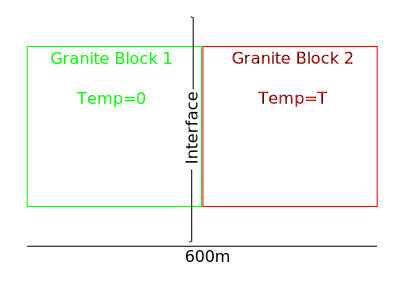
\includegraphics[width=4.in]{figures/onedheatdiff002}}
\caption{Temperature differential along a single interface between two granite blocks.}
\label{fig:onedgbmodel}
\end{figure}

By modifying our previous code it is possible to solve this new problem. In doing so we will also try to tackle a real world example and as a result, introduce and discuss some new variables. The linear model of the two blocks is very similar to the effect a large magmatic intrusion would have on a cold country rock. It is however, simpler at this stage to have both materials the same and for this example we will use granite \reffig{fig:onedgbmodel}.  The intrusion will have an initial temperature defined by \verb Tref  and the granite properties required are:
\begin{python}
#PDE related
mx = 500*m #meters - model length
my = 100*m #meters - model width
ndx = 500 # mesh steps in x direction 
ndy = 1 # mesh steps in y direction
boundloc = mx/2 # location of boundary between two blocks
q=0.*Celsius #our heat source temperature is now zero
Tref=2273.*Celsius # Kelvin -the starting temperature of our RHS Block
rho = 2750*kg/m**3 #kg/m^{3} density of granite
cp = 790.*J/(kg*K) #j/Kg.K thermal capacity
rhocp = rho*cp	#DENSITY * SPECIFIC HEAT
eta=0.  # RADIATION CONDITION
kappa=2.2*W/m/K #watts/m.K thermal conductivity
\end{python}

Since the scale and values involved in our problem have changed, the length and step size of the iteration must be considered. Instead of seconds which our units are in, it may be more prudent to decide the number of days or years we would like to run the simulation over.
\begin{python}
#Script/Iteration Related
t=0. #our start time, usually zero
tend=10*yr #the time we want to end the simulation in years
outputs = 400 # number of time steps required.
h=(tend-t)/outputs #size of time step
\end{python}

If we assume that the dimensions of the blocks are continuous and extremely large compared with the model size then we need only model a small proportion of the boundary. It is practical to locate the boundary between the two blocks at the center of our model. As there is no heat source our \verb q  variable can be set to zero. The new initial conditions are defined using the following:
\begin{python}
#establish location of boundary between two blocks
bound = x[0]-boundloc
#set initial temperature
T= 0*Tref*whereNegative(bound)+Tref*wherePositive(bound)
\end{python}
The \verb bound statement sets the boundary to the location along the \textit{x-axis} defined by \verb boundloc  .
The PDE can then be solved as before.

FOR THE READER:
\begin{enumerate}
 \item Move the boundary line between the two blocks to another part of the domain.
 \item Try splitting the domain in to multiple blocks with varying temperatures.
\end{enumerate}

